\documentclass[12pt]{article}

\usepackage[a4paper,margin=2cm]{geometry}
\usepackage{fontspec}
\usepackage{xeCJK}
\usepackage{amsmath}
\usepackage{enumitem}
\usepackage{setspace} % 設定行距
\usepackage{graphicx} % 插入圖片
\usepackage{subcaption} % 插入兩張並排圖片

\setmainfont{Times New Roman}
\setCJKmainfont[
    AutoFakeBold=3 % 設定粗體
]{DFKai-SB}

% 段落設定
\setlength{\parindent}{0pt}
\setlength{\parskip}{0.8em}
\setstretch{1.25}


%%% 文件開始
\begin{document}

\vspace*{-2cm}

%%% 頁首
\noindent
\begin{tabular*}{\textwidth}{@{\extracolsep{\fill}} l  r}
    % 左邊頁首 & 
    % 右邊頁首
\end{tabular*}

%%% 文件標題
\begin{center}
    {\LARGE\bfseries 臺南市防火宣導成果與資源配置分析報告}

    Wei-Cheng Chen\qquad{\today}
\end{center}
\vspace*{-1cm}


\section{Abstract}
本研究以臺南市消防局 107、108、109、110 與 114 年防火宣導成果資料為分析對象，從宣導規模、宣導效率、宣導對象及宣導時序等面向探討防火宣導資源配置情形。

分析結果顯示，雖然近年宣導場次與動員人次較早期年度明顯下降，但平均每場觸及人數與每位動員人員觸及人數均呈現持續成長趨勢，顯示宣導效率逐步提升。宣導對象則以學校與公共場所為主，累積觸及人次超過整體六成，反映學生族群及公共場域民眾仍為防火教育核心受眾。此外，宣導活動呈現明顯季節性特徵，其中 1 月、3 月與 9 月為主要宣導高峰期，適合作為未來人力與教材資源提前部署的重要參考。整體而言，消防局近年宣導策略已由大量分散式活動逐漸轉向較具規模且觸及範圍更廣的宣導模式，在有限資源下仍維持良好的宣導成效。


\section{研究問題}

本研究問如下：

\begin{itemize}
    \item 宣導規模是否改變？
    \item 宣導效率是否提升？
    \item 哪些族群是主要宣導對象？透過各族群累積場次與累積人次，判斷目前防火宣導資源主要集中在哪些對象。
    \item 哪些月份需要提前部署？透過月份熱圖與各月人次占比，找出宣導旺季，作為人力、場地與教材安排的參考。
\end{itemize}


\section{Methodology}


\subsection{宣導規模是否改變？}
藉由觀察年度宣導場次、宣導人次與動員人次，了解消防局在不同年度的宣導推動規模。

%%% 插入兩張並排圖片
\begin{figure}[!htbp]
    \centering

    \begin{subfigure}{0.48\textwidth}
        \centering
        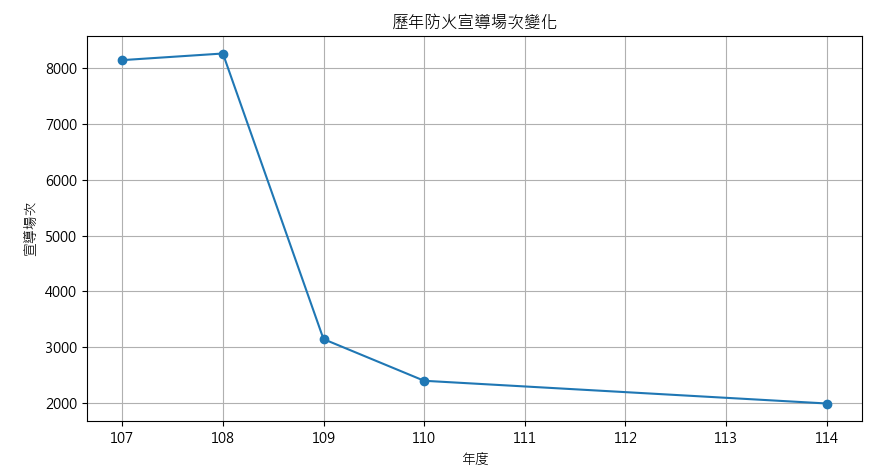
\includegraphics[width=\linewidth]{image/歷年宣導場次變化.png}
        % \caption{歷年宣導場次變化}
    \end{subfigure}
    \hfill
    \begin{subfigure}{0.48\textwidth}
        \centering
        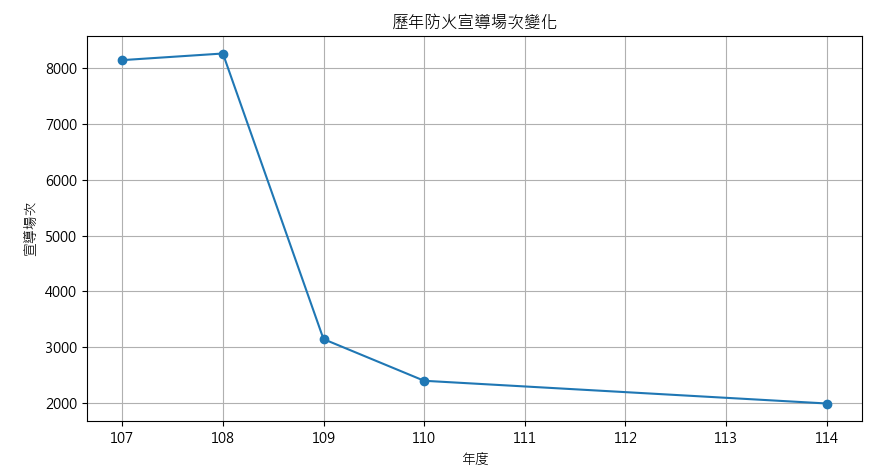
\includegraphics[width=\linewidth]{image/歷年宣導場次變化.png}
        % \caption{歷年宣導場次變化}
    \end{subfigure}
    \caption{(a). 歷年宣導場次變化 (b). 歷年宣導場次變化}
    \label{fig:歷年宣導場次變化}
\end{figure}

%%% 插入單張圖片
\begin{figure}[!htbp]
    \centering
    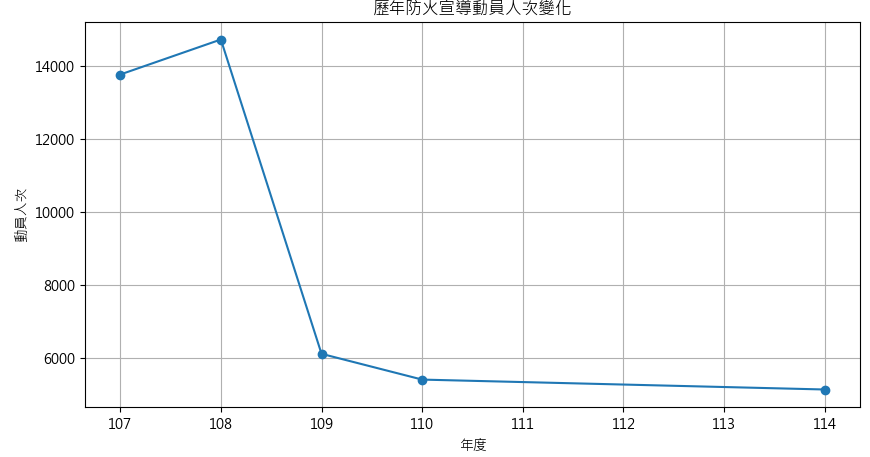
\includegraphics[width=0.8\textwidth]{image/歷年宣導動員人次變化.png}
    \caption{歷年宣導動員人次變化}
    \label{fig:歷年宣導動員人次變化}
\end{figure}


\subsection{宣導效率是否提升？}
除了總人次之外，本報告加入兩個效率指標：
\begin{itemize}
    \item 平均每場觸及人數 = 宣導人次 ÷ 宣導場次
    \item 每位動員人員觸及人數 = 宣導人次 ÷ 動員人次
\end{itemize}


研究結果如Figure~\ref{fig:平均每場觸及人數} 所表示：

第一，\textbf{平均每場觸及人數持續提升}：107 年平均每場宣導約觸及 26 人，108 年略降至 24 人左右。有趣的是，109 年之後出現明顯轉折。雖然宣導場次從八千多場大幅下降到三千多場，但每場活動接觸的人數反而增加到接近 40 人。到了 114 年更進一步提升至 75.8 人。換句話說，同樣辦一場活動，114 年接觸到的人數約為 107 年的 2.9 倍。這代表宣導方式可能已從大量、小規模、分散式活動，逐漸轉向集中式或大型宣導活動。

第二，\textbf{人力使用效率同步提升}。每位動員人員觸及人數由 107 年的 15.42 人提升至 114 年的 29.26 人。成長幅度接近1.90 倍。也就是說，114 年每投入一位宣導人員，所能接觸的民眾數量幾乎是 107 年的兩倍。從管理角度來看，代表有限的人力資源能產生更大的宣導效益。

第三，\textbf{規模下降不代表績效下降}。若只觀察宣導場次：107年為8149場，而114年為1984場。看起來減少超過七成。但加入效率指標後可以發現每場宣導觸及人數持續增加，且每位人員影響力持續增加。因此不能僅以宣導場次作為績效判斷依據。也可以推測消防局近年較可能採用「減少活動數量、提高單場規模」的宣導策略，使整體資源投入更加集中。

%%% 插入兩張並排圖片
\begin{figure}[!htbp]
    \centering

    \begin{subfigure}{0.48\textwidth}
        \centering
        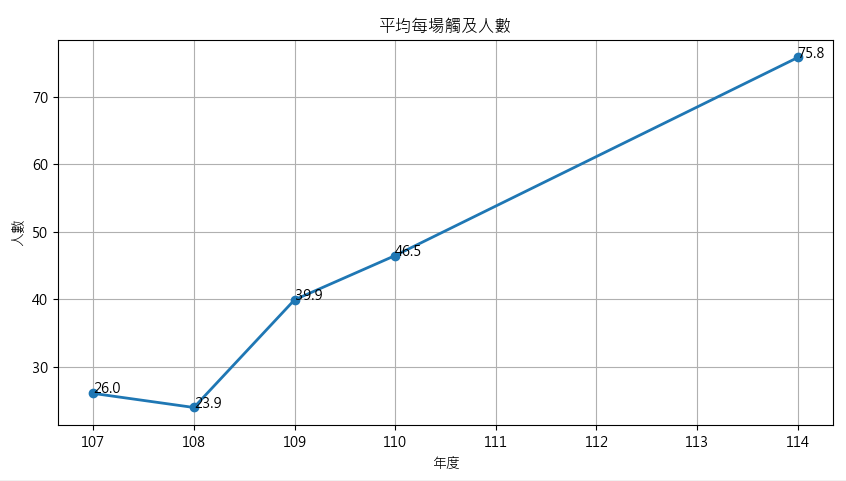
\includegraphics[width=\linewidth]{image/平均每場觸及人數.png}
        % \caption{平均每場觸及人數}
    \end{subfigure}
    \hfill
    \begin{subfigure}{0.48\textwidth}
        \centering
        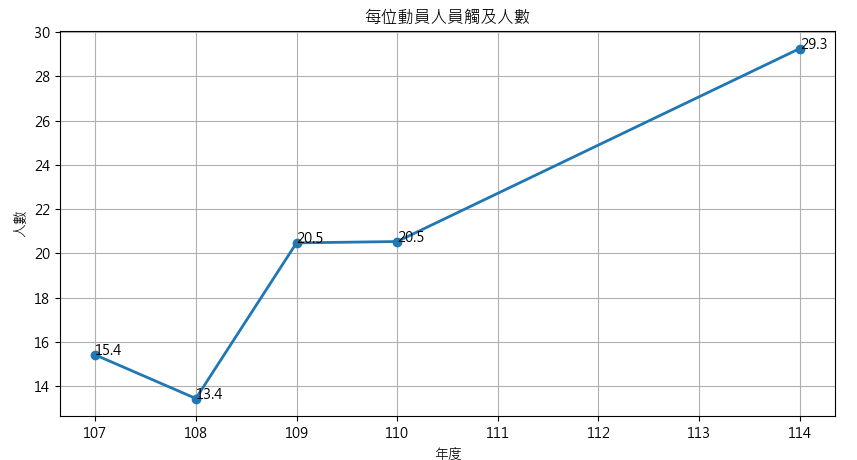
\includegraphics[width=\linewidth]{image/每位動員人員觸及人數.png}
        % \caption{每位動員人員觸及人數}
    \end{subfigure}
    \caption{(a). 平均每場觸及人數 (b). 每位動員人員觸及人數}
    \label{fig:平均每場觸及人數}
\end{figure}



\subsection{哪些族群是主要宣導對象}

分析結果顯示，防火宣導資源主要集中在「學校」與「公共場所」兩大族群。從累積宣導人次來看，學校共觸及 312,098 人次，占整體 37.84\%；公共場所共觸及 241,056人次，占 29.22\%。兩者合計已超過整體宣導人次的六成，代表消防局的宣導策略明顯以學生族群與公共場域民眾為主要對象。

回頭看場次分布，社區鄰里與其它類別的場次較多，分別達 5,785 場與 5,984 場，但累積人次並未高於學校與公共場所。這代表社區鄰里宣導可能較偏向小規模、分散式接觸；學校與公共場所則較容易在單次活動中接觸大量民眾。因此，若從「觸及人次」判斷主要宣導對象，學校與公共場所是目前防火宣導最核心的兩個族群；若從「宣導場次」觀察，社區鄰里與其它類別則承擔較多基層、分散型宣導任務。這也說明消防局的宣導資源並非只集中在單一場域，而是同時兼顧大量觸及與社區滲透兩種策略。

%%% 插入兩張並排圖片
\begin{figure}[!htbp]
    \centering

    \begin{subfigure}{0.48\textwidth}
        \centering
        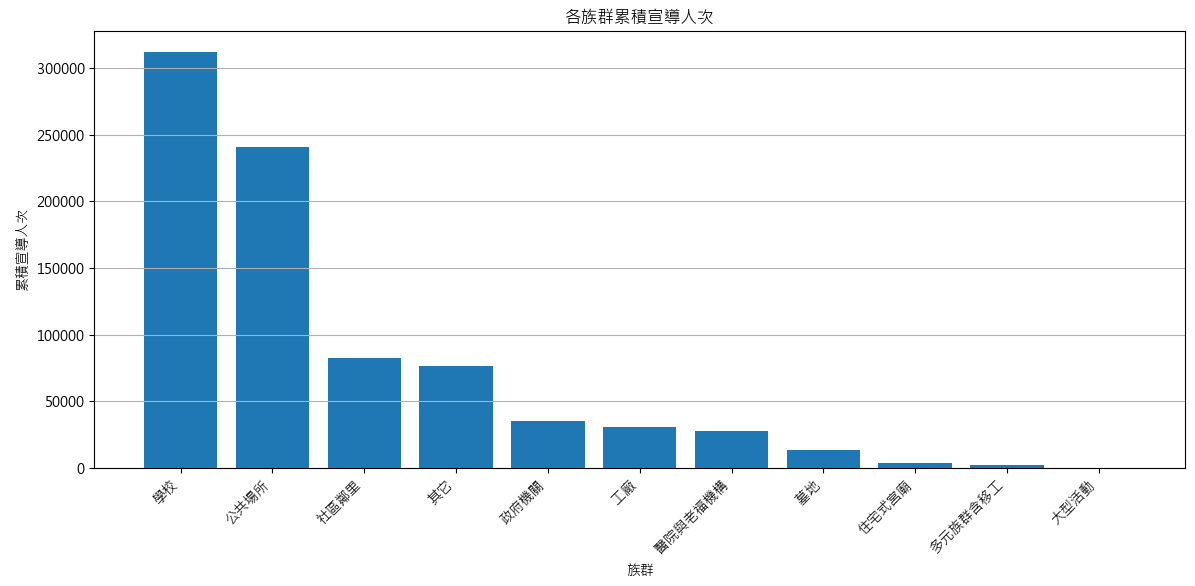
\includegraphics[width=\linewidth]{image/各族群累積宣導人次.png}
        % \caption{歷年宣導場次變化}
    \end{subfigure}
    \hfill
    \begin{subfigure}{0.48\textwidth}
        \centering
        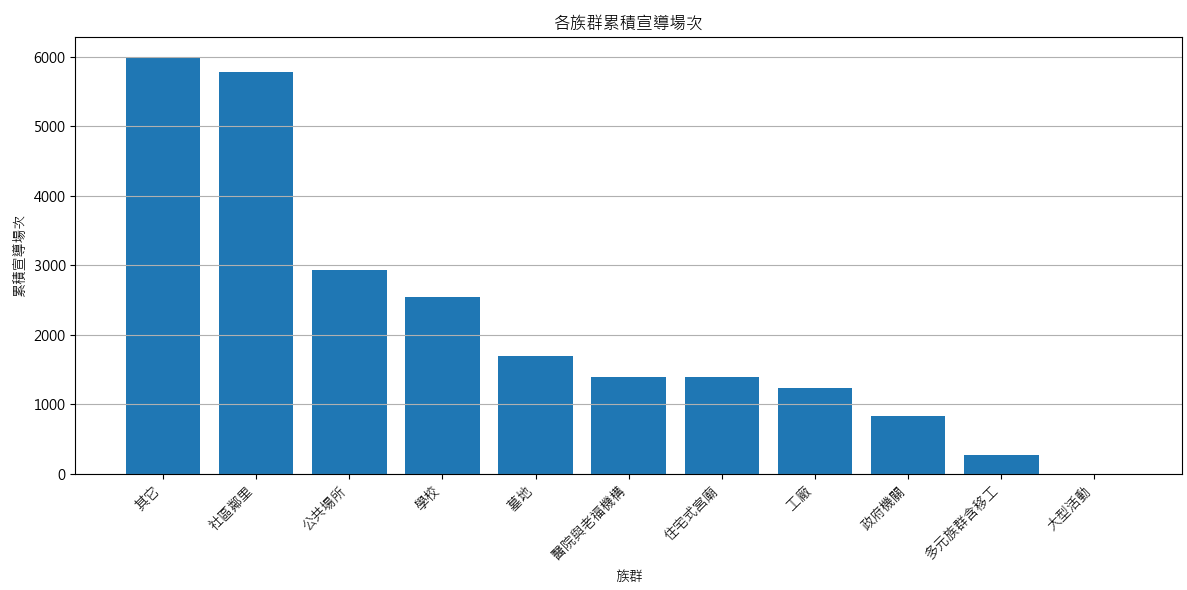
\includegraphics[width=\linewidth]{image/各族群累積宣導場次.png}
        % \caption{歷年宣導場次變化}
    \end{subfigure}
    \caption{(a). 各族群累積宣導人次 (b). 各族群累積宣導場次}
    \label{fig:各族群累積宣導人次}
\end{figure}

%%% 插入單張圖片
\begin{figure}[!htbp]
    \centering
    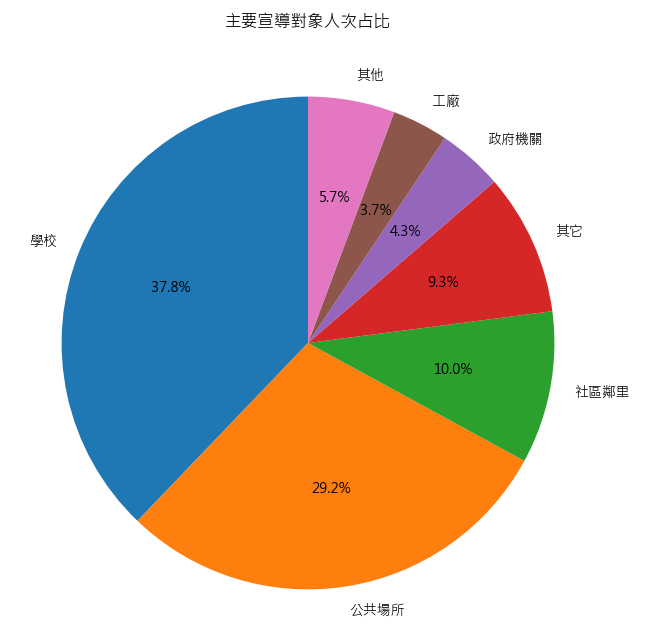
\includegraphics[width=0.6\textwidth]{image/主要宣導對象人次占比.png}
    \caption{主要宣導對象人次占比}
    \label{fig:主要宣導對象人次占比}
\end{figure}


\subsection{哪些月份需要提前部署}
分析結果顯示，防火宣導具有明顯的月份集中現象。從累積宣導人次觀察，1 月為最主要的宣導高峰，共觸及 142,963 人次，占整體 17.94\%；3 月與 9 月也相當突出，分別占 12.74\% 與 12.71\%。這三個月份合計已超過整體宣導人次四成，代表消防局在年初、春季開學後，以及秋季開學期間投入較多宣導資源。

從熱圖來看，1 月幾乎在多數年度都有較高宣導人次，顯示年初可能是防火宣導的重要部署期。3 月與 9 月則可能與學校行事曆有關，學生族群集中、場地容易安排，也讓單次活動能觸及較多人。相較之下，7 月、8 月的人次偏低，暑假期間學校宣導條件較弱，宣導熱度也明顯下降。

因此，若要提前規劃人力、場地與教材，建議將 1 月、3 月、9 月列為主要宣導旺季。其中 1 月應提前在前一年度 12 月完成教材與人力排班；3 月與 9 月則可配合學校開學時程，提前與校方或公共場所協調宣導場次。這樣安排可以避免旺季臨時調度，也能讓宣導資源更集中地發揮效果。

%%% 插入單張圖片
\begin{figure}[!htbp]
    \centering
    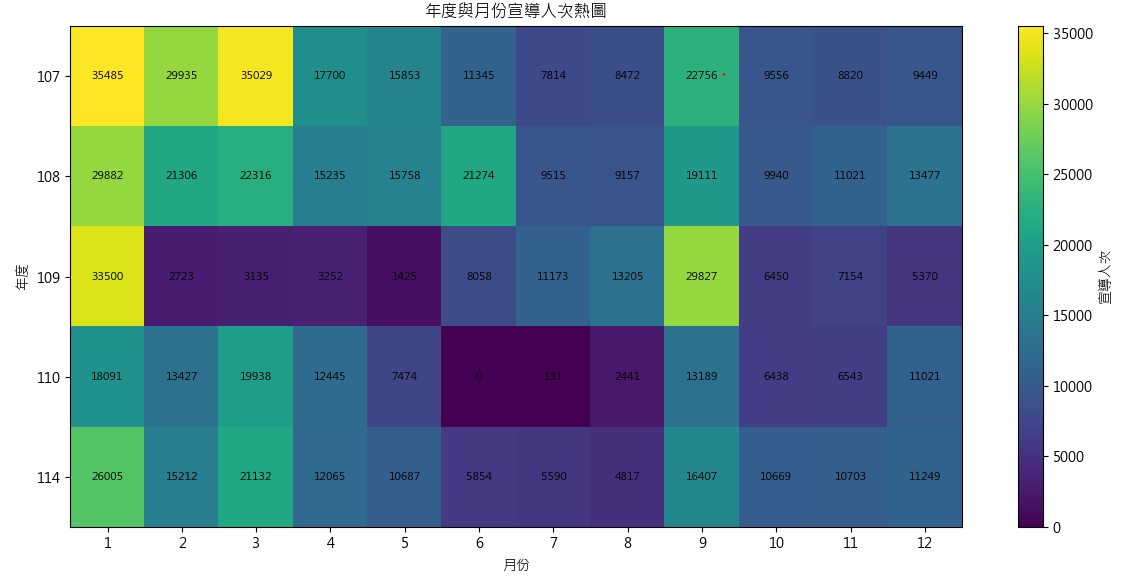
\includegraphics[width=0.9\textwidth]{image/熱圖.png}
    \caption{熱圖}
    \label{fig:熱圖}
\end{figure}

%%% 插入單張圖片
\begin{figure}[!htbp]
    \centering
    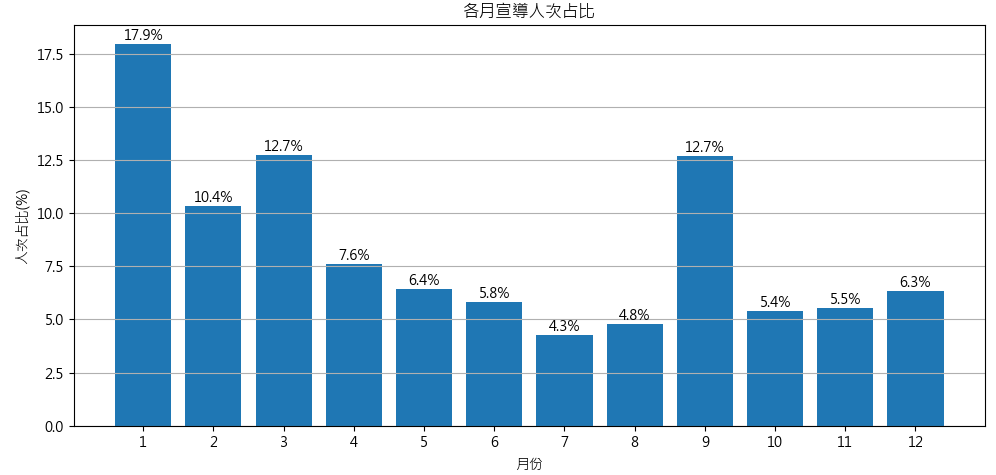
\includegraphics[width=0.7\textwidth]{image/個月宣導人次占比.png}
    \caption{個月宣導人次占比}
    \label{fig:主要宣導對象人次占比}
\end{figure}


\section{Conclusion}

本研究透過臺南市消防局歷年防火宣導成果資料，分析宣導規模、宣導效率、宣導對象及宣導時序等面向，以了解防火宣導資源的運用情形。

分析結果顯示，107 年至 108 年為防火宣導規模較大的時期，無論在宣導場次、宣導人次或動員人次方面皆維持較高水準。109 年以後，宣導場次與動員人次明顯下降，但宣導人次下降幅度相對較小，顯示消防局在資源投入減少的情況下，仍維持一定程度的宣導觸及能力。

從效率面觀察，平均每場觸及人數由 107 年的 26 人提升至 114 年的 75.8 人，每位動員人員觸及人數亦由 15.42 人提升至 29.26 人。這顯示近年防火宣導逐漸由大量、小規模活動轉向較具規模且觸及範圍較廣的宣導模式，人力與資源運用效率皆有提升。

在宣導對象方面，學校與公共場所為最主要的宣導場域，累積觸及人次超過整體六成。其中學校族群占比最高，顯示學生仍是目前防火教育推廣的重要目標族群。另一方面，社區鄰里雖然宣導場次較多，但單場觸及人數相對較少，反映其具有深入基層、分散接觸的特性。

從月份分布來看，防火宣導具有明顯的季節性特徵。1 月、3 月及 9 月的宣導人次明顯高於其他月份，顯示年初以及春、秋兩次開學期間為防火宣導的重要推動時機。這些月份不僅是宣導需求較高的時段，也是資源配置與活動規劃的重要參考依據。

整體而言，臺南市消防局近年已逐步由「擴大宣導規模」轉向「提升宣導效益」的推動模式。在有限人力與資源條件下，宣導效率與觸及能力皆呈現正向發展，未來若能結合成效評估機制與精準資源配置策略，將有助於進一步提升防火宣導工作的整體成效。

%%% 文件結束
\end{document}